\section{Introducción Teórica}
%Contendrá una breve explicación de la base teórica que fundamenta los métodos involu- crados en el
%trabajo, junto con los métodos mismos. No deben incluirse demostraciones de propiedades ni
%teoremas, ejemplos innecesarios, ni definiciones elementales (como por ejemplo la de matriz
%simétrica). En vez de definiciones básicas es conveniente citar ejemplos de bibliografía adecuada.
%Una cita vale más que mil palabras.
%
Dado un horno industrial de gran tamaño, se estudia en este trabajo la búsqueda de una isoterma dada
en las paredes de éste. Dado que computacionalmente es imposible analizar el problema para
dimensiones continuas para la pared, se lo discretiza según información dada. Esta información
requerida del horno sería el radio en la parte interna de la pared, la cantidad de ángulos en el cual
discretizarlo, el radio en la parte externa de la pared, la temperatura interna, la temperatura
externa y la isoterma buscada. Se adjunta un gráfico para verlo con más claridad.

\begin{figure}[ht]
  \begin {center}
    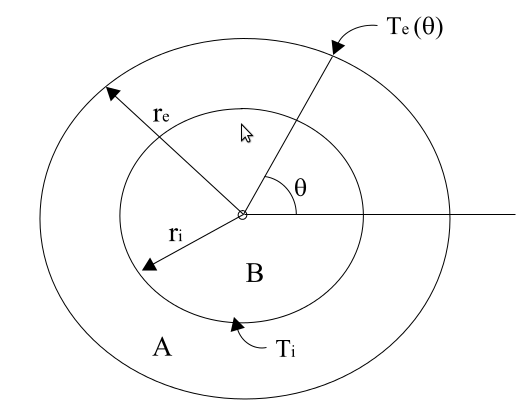
\includegraphics[width=0.6\columnwidth]{Horno.png}
    \caption{Sección circular del horno}
  \end{center}
\end{figure}

Para lograr lo pedido, en nos enfocamos en la resolución de sistemas matriciales del tipo $Ax=b$,
donde $A$ es una matriz inversible con coeficientes reales. El método clásico por excelencia para
este tipo de problemas es la eliminación gaussiana que básicamente consiste en aplicar operaciones
elementales de fila sobre la matriz $A$ y el vector $b$ para poder simplificar el sistema de
ecuaciones original, obteniéndose un sistema triangulado que puede ser fácilmente resuelto aplicando
un algoritmo de sustitución hacia atrás \cite[6.1]{burden}. La eliminación gaussiana original puede
(y en algunas ocasiones debe) realizar permutaciones de filas, pero como vamos a restringir nuestro
estudio a matrices diagonal dominantes (para más información, ver demostración en el apéndice), se
omitirá el pivoteo, y cada vez que se haga mención a dicho algoritmo se entenderá que es sin
pivoteo.

El otro método estudiado en este informe es la factorización LU, que básicamente consiste en hallar
una forma de $A$ que sea igual a $L$ $\cdot$ $U$, donde $U$ es triangular superior y $L$ triangular
inferior, de esta manera $Ax=b$ se convierte en $LUx=b$, y si consideramos $y=Ux$, la solución al
sistema puede hallarse resolviendo primero $Ly=b$, y luego $Ux=y$. Esta factorización permite evitar
tener que triangular la matriz $A$, cada vez que $b$ es modificado \cite[6.5]{burden}.
